\documentclass[11pt,ignorenonframetext,]{beamer}
\setbeamertemplate{caption}[numbered]
\setbeamertemplate{caption label separator}{: }
\setbeamercolor{caption name}{fg=normal text.fg}
\beamertemplatenavigationsymbolsempty
\usepackage{lmodern}
\usepackage{amssymb,amsmath}
\usepackage{ifxetex,ifluatex}
\usepackage{fixltx2e} % provides \textsubscript
\ifnum 0\ifxetex 1\fi\ifluatex 1\fi=0 % if pdftex
  \usepackage[T1]{fontenc}
  \usepackage[utf8]{inputenc}
\else % if luatex or xelatex
  \ifxetex
    \usepackage{mathspec}
  \else
    \usepackage{fontspec}
  \fi
  \defaultfontfeatures{Ligatures=TeX,Scale=MatchLowercase}
\fi
\usetheme[]{metropolis}
% use upquote if available, for straight quotes in verbatim environments
\IfFileExists{upquote.sty}{\usepackage{upquote}}{}
% use microtype if available
\IfFileExists{microtype.sty}{%
\usepackage{microtype}
\UseMicrotypeSet[protrusion]{basicmath} % disable protrusion for tt fonts
}{}
\newif\ifbibliography
\hypersetup{
            pdftitle={Lecture 20},
            pdfauthor={Colin Rundel},
            pdfborder={0 0 0},
            breaklinks=true}
\urlstyle{same}  % don't use monospace font for urls
\usepackage{color}
\usepackage{fancyvrb}
\newcommand{\VerbBar}{|}
\newcommand{\VERB}{\Verb[commandchars=\\\{\}]}
\DefineVerbatimEnvironment{Highlighting}{Verbatim}{commandchars=\\\{\}}
% Add ',fontsize=\small' for more characters per line
\newenvironment{Shaded}{}{}
\newcommand{\KeywordTok}[1]{\textcolor[rgb]{0.00,0.44,0.13}{\textbf{#1}}}
\newcommand{\DataTypeTok}[1]{\textcolor[rgb]{0.56,0.13,0.00}{#1}}
\newcommand{\DecValTok}[1]{\textcolor[rgb]{0.25,0.63,0.44}{#1}}
\newcommand{\BaseNTok}[1]{\textcolor[rgb]{0.25,0.63,0.44}{#1}}
\newcommand{\FloatTok}[1]{\textcolor[rgb]{0.25,0.63,0.44}{#1}}
\newcommand{\ConstantTok}[1]{\textcolor[rgb]{0.53,0.00,0.00}{#1}}
\newcommand{\CharTok}[1]{\textcolor[rgb]{0.25,0.44,0.63}{#1}}
\newcommand{\SpecialCharTok}[1]{\textcolor[rgb]{0.25,0.44,0.63}{#1}}
\newcommand{\StringTok}[1]{\textcolor[rgb]{0.25,0.44,0.63}{#1}}
\newcommand{\VerbatimStringTok}[1]{\textcolor[rgb]{0.25,0.44,0.63}{#1}}
\newcommand{\SpecialStringTok}[1]{\textcolor[rgb]{0.73,0.40,0.53}{#1}}
\newcommand{\ImportTok}[1]{#1}
\newcommand{\CommentTok}[1]{\textcolor[rgb]{0.38,0.63,0.69}{\textit{#1}}}
\newcommand{\DocumentationTok}[1]{\textcolor[rgb]{0.73,0.13,0.13}{\textit{#1}}}
\newcommand{\AnnotationTok}[1]{\textcolor[rgb]{0.38,0.63,0.69}{\textbf{\textit{#1}}}}
\newcommand{\CommentVarTok}[1]{\textcolor[rgb]{0.38,0.63,0.69}{\textbf{\textit{#1}}}}
\newcommand{\OtherTok}[1]{\textcolor[rgb]{0.00,0.44,0.13}{#1}}
\newcommand{\FunctionTok}[1]{\textcolor[rgb]{0.02,0.16,0.49}{#1}}
\newcommand{\VariableTok}[1]{\textcolor[rgb]{0.10,0.09,0.49}{#1}}
\newcommand{\ControlFlowTok}[1]{\textcolor[rgb]{0.00,0.44,0.13}{\textbf{#1}}}
\newcommand{\OperatorTok}[1]{\textcolor[rgb]{0.40,0.40,0.40}{#1}}
\newcommand{\BuiltInTok}[1]{#1}
\newcommand{\ExtensionTok}[1]{#1}
\newcommand{\PreprocessorTok}[1]{\textcolor[rgb]{0.74,0.48,0.00}{#1}}
\newcommand{\AttributeTok}[1]{\textcolor[rgb]{0.49,0.56,0.16}{#1}}
\newcommand{\RegionMarkerTok}[1]{#1}
\newcommand{\InformationTok}[1]{\textcolor[rgb]{0.38,0.63,0.69}{\textbf{\textit{#1}}}}
\newcommand{\WarningTok}[1]{\textcolor[rgb]{0.38,0.63,0.69}{\textbf{\textit{#1}}}}
\newcommand{\AlertTok}[1]{\textcolor[rgb]{1.00,0.00,0.00}{\textbf{#1}}}
\newcommand{\ErrorTok}[1]{\textcolor[rgb]{1.00,0.00,0.00}{\textbf{#1}}}
\newcommand{\NormalTok}[1]{#1}
\usepackage{graphicx,grffile}
\makeatletter
\def\maxwidth{\ifdim\Gin@nat@width>\linewidth\linewidth\else\Gin@nat@width\fi}
\def\maxheight{\ifdim\Gin@nat@height>\textheight0.8\textheight\else\Gin@nat@height\fi}
\makeatother
% Scale images if necessary, so that they will not overflow the page
% margins by default, and it is still possible to overwrite the defaults
% using explicit options in \includegraphics[width, height, ...]{}
\setkeys{Gin}{width=\maxwidth,height=\maxheight,keepaspectratio}

% Prevent slide breaks in the middle of a paragraph:
\widowpenalties 1 10000
\raggedbottom

\AtBeginPart{
  \let\insertpartnumber\relax
  \let\partname\relax
  \frame{\partpage}
}
\AtBeginSection{
  \ifbibliography
  \else
    \let\insertsectionnumber\relax
    \let\sectionname\relax
    \frame{\sectionpage}
  \fi
}
\AtBeginSubsection{
  \let\insertsubsectionnumber\relax
  \let\subsectionname\relax
  \frame{\subsectionpage}
}

\setlength{\parindent}{0pt}
\setlength{\parskip}{6pt plus 2pt minus 1pt}
\setlength{\emergencystretch}{3em}  % prevent overfull lines
\providecommand{\tightlist}{%
  \setlength{\itemsep}{0pt}\setlength{\parskip}{0pt}}
\setcounter{secnumdepth}{0}

\usepackage{geometry}
\usepackage{graphicx}
\usepackage{amssymb}
\usepackage{color}          	% gives color options
\usepackage{url}		% produces hyperlinks
\usepackage[english]{babel}
\usepackage{colortbl}	% allows for color usage in tables
\usepackage{multirow}	% allows for rows that span multiple rows in tables
\usepackage{xcolor}		% this package has a variety of color options
\usepackage{calc}
\usepackage{multicol}
\usepackage{wrapfig}
\usepackage{textcomp}
\usepackage{bm}
\usepackage{bbm}
\usepackage{setspace}
\usepackage{changepage}
\singlespacing

\usepackage{fontspec}
\newfontfamily\DejaSans{DejaVu Sans}

%%%%%%%%%%%%%%%%
% Small code output
%%%%%%%%%%%%%%%%

%% change fontsize of R code

\makeatletter
\@ifundefined{Shaded}{\newenvironment{Shaded}{}{}}{}
\makeatother


\let\oldShaded\Shaded
\let\endoldShaded\endShaded
\renewenvironment{Shaded}{\footnotesize\begin{spacing}{0.9}\oldShaded}{\endoldShaded\end{spacing}}

%% change fontsize of output
\let\oldverbatim\verbatim
\let\endoldverbatim\endverbatim
\renewenvironment{verbatim}{\footnotesize\begin{spacing}{0.9}\oldverbatim}{\endoldverbatim\end{spacing}}


\newcommand{\tinyoutput}{
  \renewenvironment{Shaded}{\tiny\begin{spacing}{0.9}\oldShaded}{\endoldShaded\end{spacing}}
  \renewenvironment{verbatim}{\tiny\begin{spacing}{0.9}\oldverbatim}{\endoldverbatim\end{spacing}}
}

\newcommand{\scriptoutput}{
  \renewenvironment{Shaded}{\scriptsize\begin{spacing}{0.9}\oldShaded}{\endoldShaded\end{spacing}}
  \renewenvironment{verbatim}{\scriptsize\begin{spacing}{0.9}\oldverbatim}{\endoldverbatim\end{spacing}}
}

\newcommand{\footnoteoutput}{
  \renewenvironment{Shaded}{\footnotesize\begin{spacing}{0.9}\oldShaded}{\endoldShaded\end{spacing}}
  \renewenvironment{verbatim}{\footnotesize\begin{spacing}{0.9}\oldverbatim}{\endoldverbatim\end{spacing}}
}

%\newcommand{\verbatimfont}[1]{\renewcommand{\verbatim@font}{\ttfamily#1}}


%%%%%%%%%%%%%%%%
% Custom Colors
%%%%%%%%%%%%%%%%

\xdefinecolor{oiBlue}{rgb}{0.15, 0.35, 0.55}
\xdefinecolor{gray}{rgb}{0.5, 0.5, 0.5}
\xdefinecolor{darkGray}{rgb}{0.3, 0.3, 0.3}
\xdefinecolor{darkerGray}{rgb}{0.2, 0.2, 0.2}
\xdefinecolor{rubineRed}{rgb}{0.89,0,0.30}
\xdefinecolor{linkCol}{rgb}{0.11,0.49,0.95}	
\xdefinecolor{irishGreen}{rgb}{0,0.60,0}	
\xdefinecolor{darkturquoise}{rgb}{0.44, 0.58, 0.86}
\definecolor{lightGreen}{rgb}{0.533,0.765,0.42}
%\xdefinecolor{hlblue}{rgb}{0.051,0.65,1}
\xdefinecolor{hlblue}{rgb}{ 0.055, 0.639, 0.831}
\definecolor{light}{rgb}{.337,.608,.741}
\definecolor{dark}{rgb}{.337,.608,.741}

\definecolor{cpink}{rgb}{0.93, 0.23, 0.51}

%%%%%%%%%%%%%%%%
% Custom Commands
%%%%%%%%%%%%%%%%

% text colors
\newcommand{\red}[1]{\textit{\textcolor{rubineRed}{#1}}}
\newcommand{\orange}[1]{\textit{\textcolor{orange}{#1}}}
\newcommand{\pink}[1]{\textit{\textcolor{rubineRed!90!white!50}{#1}}}
\newcommand{\green}[1]{\textit{\textcolor{irishGreen}{#1}}}
\newcommand{\blue}[1]{\textit{\textcolor{darkturquoise}{#1}}}
\newcommand{\light}[1]{\textcolor{light}{\textbf{#1}}}
\newcommand{\dark}[1]{\textcolor{dark}{#1}}
\newcommand{\gray}[1]{\textcolor{gray}{#1}}


% links: webURL, webLin, appLink
\newcommand{\webURL}[1]{\urlstyle{same}{\textit{\textcolor{linkCol}{\url{#1}}} }}
\newcommand{\webLink}[2]{\href{#1}{\textcolor{linkCol}{{#2}}}}
\newcommand{\appLink}[2]{\href{#1}{\textcolor{lightGreen!80!black!90}{{#2}}}}

% mail
\newcommand{\mail}[1]{\href{mailto:#1}{\textit{\textcolor{linkCol}{#1}}}}

% highlighting: hl, hlGr, mathhl
\newcommand{\hl}[1]{\textit{\textcolor{hlblue}{#1}}}
\newcommand{\hlGr}[1]{\textit{\textcolor{lightGreen}{#1}}}
\newcommand{\hlRd}[1]{\textit{\textcolor{rubineRed}{#1}}}
\newcommand{\mathhl}[1]{\textcolor{hlblue}{\ensuremath{#1}}}

% example
\newcommand{\ex}[1]{\textcolor{blue}{{{\small (#1)}}}}


\DeclareMathOperator*{\argmin}{arg\,min}
\DeclareMathOperator*{\argmax}{arg\,max}

\title{Lecture 20}
\subtitle{Spatial Random Effects Models + Point Reference Spatial Data}
\author{Colin Rundel}
\date{04/03/2017}

\begin{document}
\frame{\titlepage}

\section{Spatial Random Effects
Models}\label{spatial-random-effects-models}

\begin{frame}{Scottish Lip Cancer Data}

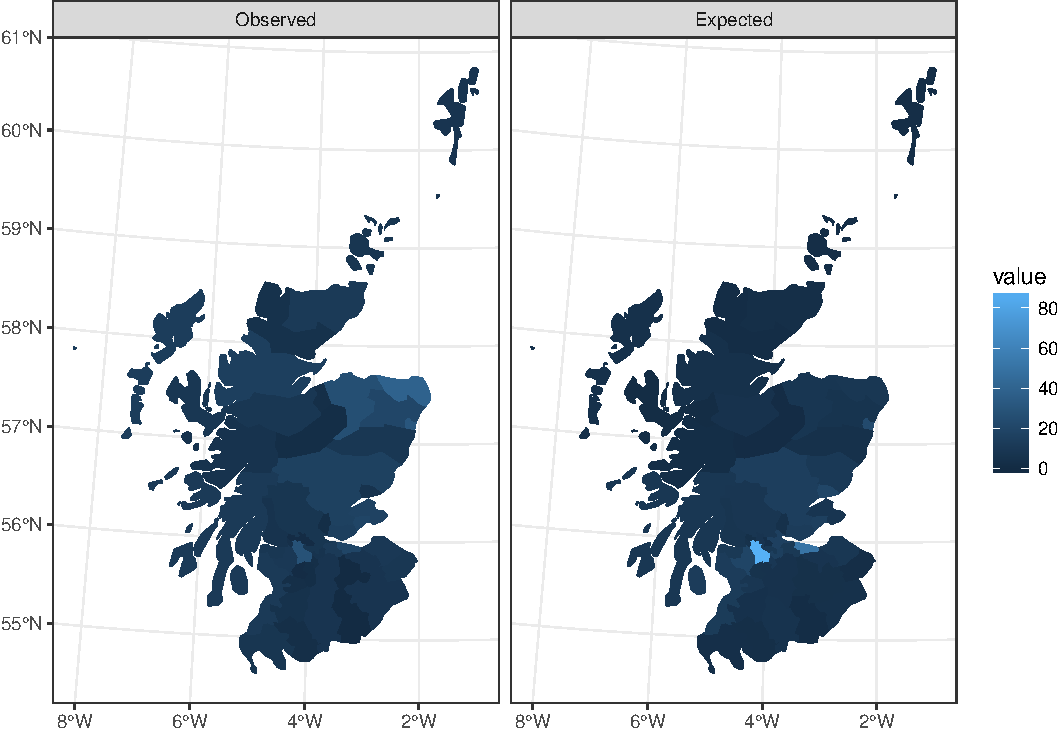
\includegraphics{Lec20_files/figure-beamer/unnamed-chunk-1-1.pdf}

\end{frame}

\begin{frame}{}

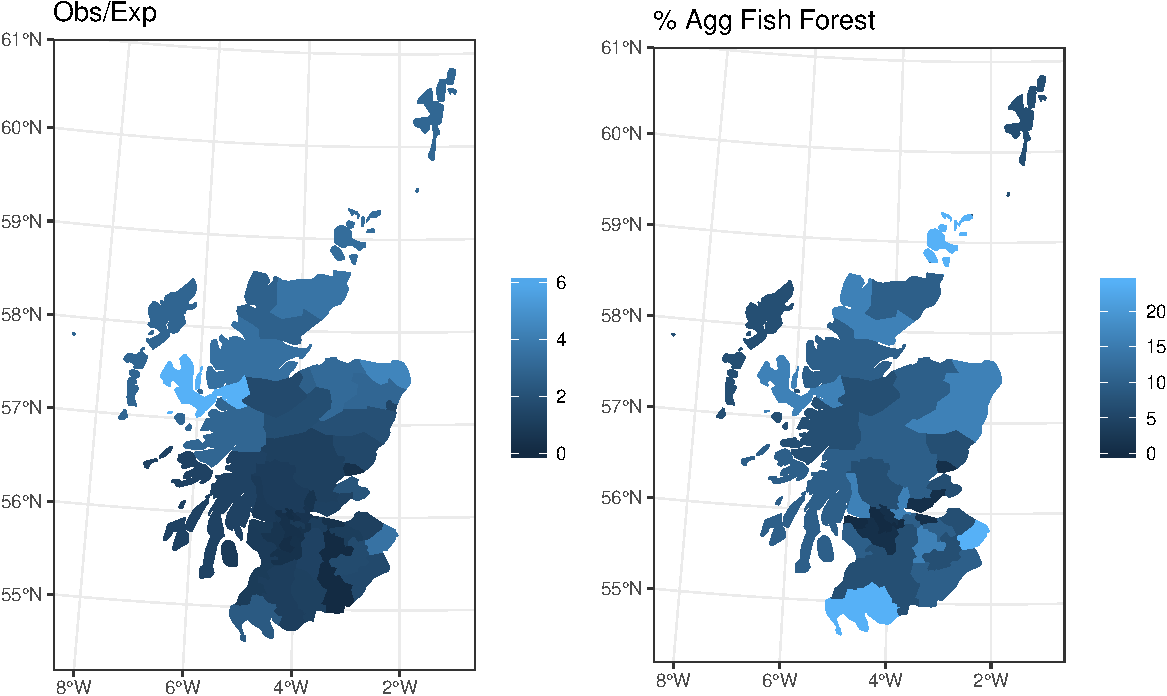
\includegraphics{Lec20_files/figure-beamer/unnamed-chunk-2-1.pdf}

\end{frame}

\begin{frame}{Neighborhood / weight matrix}

\vspace{-4mm}

\begin{center}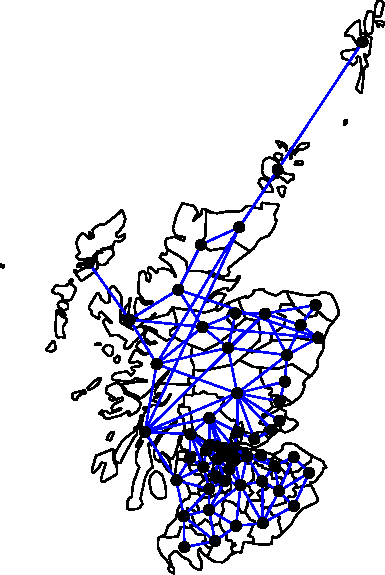
\includegraphics[height=\textheight]{Lec20_files/figure-beamer/unnamed-chunk-3-1} \end{center}

\end{frame}

\begin{frame}[fragile]{Moran's I}

\scriptoutput

\begin{Shaded}
\begin{Highlighting}[]
\NormalTok{morans_I =}\StringTok{ }\ControlFlowTok{function}\NormalTok{(y, w)}
\NormalTok{\{}
\NormalTok{  n =}\StringTok{ }\KeywordTok{length}\NormalTok{(y)}
\NormalTok{  y_bar =}\StringTok{ }\KeywordTok{mean}\NormalTok{(y)}
\NormalTok{  num =}\StringTok{ }\KeywordTok{sum}\NormalTok{(w }\OperatorTok{*}\StringTok{ }\NormalTok{(y}\OperatorTok{-}\NormalTok{y_bar) }\OperatorTok\StringTok{ }\KeywordTok{t}\NormalTok{(y}\OperatorTok{-}\NormalTok{y_bar))  }
\NormalTok{  denom =}\StringTok{ }\KeywordTok{sum}\NormalTok{( (y}\OperatorTok{-}\NormalTok{y_bar)}\OperatorTok{^}\DecValTok{2}\NormalTok{ )}
\NormalTok{  (n}\OperatorTok{/}\KeywordTok{sum}\NormalTok{(w)) }\OperatorTok{*}\StringTok{ }\NormalTok{(num}\OperatorTok{/}\NormalTok{denom)}
\NormalTok{\}}

\KeywordTok{morans_I}\NormalTok{(}\DataTypeTok{y =}\NormalTok{ lip_cancer}\OperatorTok{$}\NormalTok{Observed, }\DataTypeTok{w =} \KeywordTok{diag}\NormalTok{(}\KeywordTok{rowSums}\NormalTok{(W)) }\OperatorTok\StringTok{ }\NormalTok{W)}
\NormalTok{## [1] 0.2258758}

\KeywordTok{morans_I}\NormalTok{(}\DataTypeTok{y =}\NormalTok{ lip_cancer}\OperatorTok{$}\NormalTok{Observed }\OperatorTok{/}\StringTok{ }\NormalTok{lip_cancer}\OperatorTok{$}\NormalTok{Expected, }
         \DataTypeTok{w =} \KeywordTok{diag}\NormalTok{(}\KeywordTok{rowSums}\NormalTok{(W)) }\OperatorTok\StringTok{ }\NormalTok{W)}
\NormalTok{## [1] 0.5323161}

\NormalTok{ape}\OperatorTok{::}\KeywordTok{Moran.I}\NormalTok{(lip_cancer}\OperatorTok{$}\NormalTok{Observed }\OperatorTok{/}\StringTok{ }\NormalTok{lip_cancer}\OperatorTok{$}\NormalTok{Expected, }
             \DataTypeTok{weight =} \KeywordTok{diag}\NormalTok{(}\KeywordTok{rowSums}\NormalTok{(W)) }\OperatorTok\StringTok{ }\NormalTok{W) }\OperatorTok\StringTok{ }\KeywordTok{str}\NormalTok{()}
\NormalTok{## List of 4}
\NormalTok{##  $ observed: num 0.666}
\NormalTok{##  $ expected: num -0.0182}
\NormalTok{##  $ sd      : num 0.0784}
\NormalTok{##  $ p.value : num 0}
\end{Highlighting}
\end{Shaded}

\end{frame}

\begin{frame}[t]{A hierachical model for lip cancer}

We have observed counts of lip cancer for 56 districts in Scotland. Let
\(y_i\) represent the number of lip cancer for district \(i\).

\[\begin{aligned}
y_i &\sim \text{Poisson}(\lambda_i) \\
\\
\log(\lambda_i) &= \log(E_i) + x_i \beta + \omega_i \\
\\
\bm\omega &\sim \mathcal{N}(\bm{0},~\sigma^2(\bm{D}-\phi\,\bm{W})^{-1})
\end{aligned}\]

where \(E_i\) is the expected counts for each region (and serves as an
offet).

\end{frame}

\begin{frame}[fragile]{Data prep \& JAGS model}

\scriptoutput

\begin{Shaded}
\begin{Highlighting}[]
\NormalTok{D =}\StringTok{ }\KeywordTok{diag}\NormalTok{(}\KeywordTok{rowSums}\NormalTok{(W))}
\NormalTok{X =}\StringTok{ }\KeywordTok{model.matrix}\NormalTok{(}\OperatorTok{~}\KeywordTok{scale}\NormalTok{(lip_cancer}\OperatorTok{$}\NormalTok{pcaff))}
\NormalTok{log_offset =}\StringTok{ }\KeywordTok{log}\NormalTok{(lip_cancer}\OperatorTok{$}\NormalTok{Expected)}
\NormalTok{y =}\StringTok{ }\NormalTok{lip_cancer}\OperatorTok{$}\NormalTok{Observed}
\end{Highlighting}
\end{Shaded}

\begin{verbatim}
## model{
##   for(i in 1:length(y)) {
##     y[i] ~ dpois(lambda[i])
##     y_pred[i] ~ dpois(lambda[i])
##     log(lambda[i]) <- log_offset[i] + X[i,] %*% beta + omega[i]
##   }
## 
##   for(i in 1:2) {
##     beta[i] ~ dnorm(0,1)
##   }
## 
##   omega ~ dmnorm(rep(0,length(y)), tau * (D - phi*W))
##   sigma2 <- 1/tau
##   tau ~ dgamma(2, 2)
##   phi ~ dunif(0,0.99)
## }
\end{verbatim}

\end{frame}

\begin{frame}{Model Results}

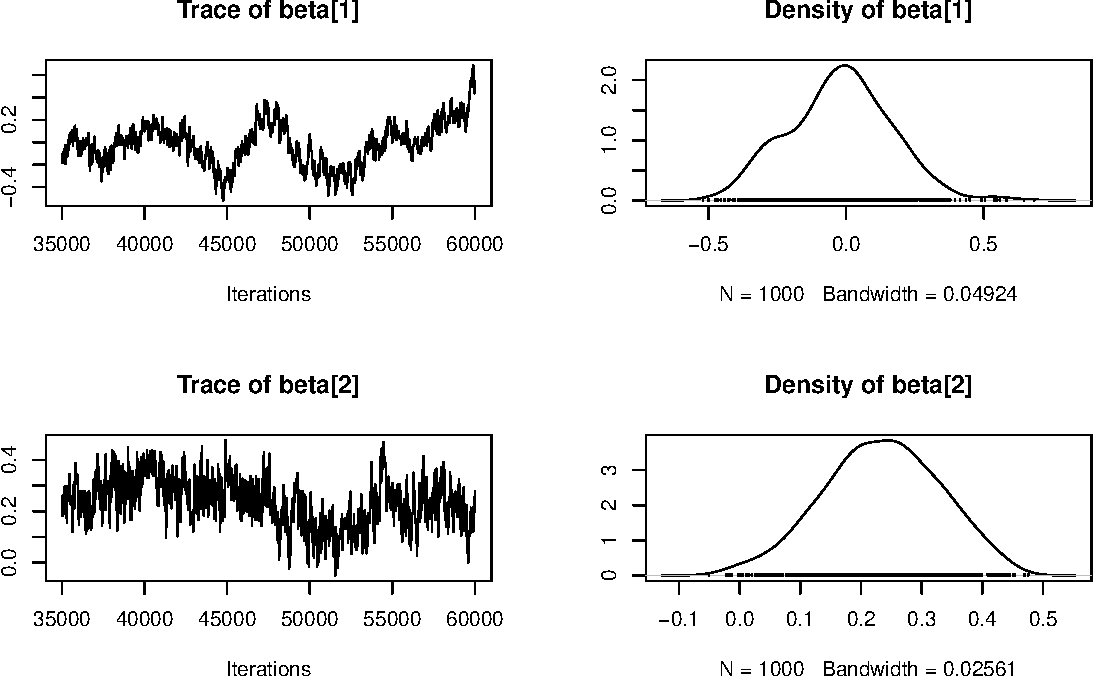
\includegraphics{Lec20_files/figure-beamer/unnamed-chunk-8-1.pdf}

\end{frame}

\begin{frame}{}

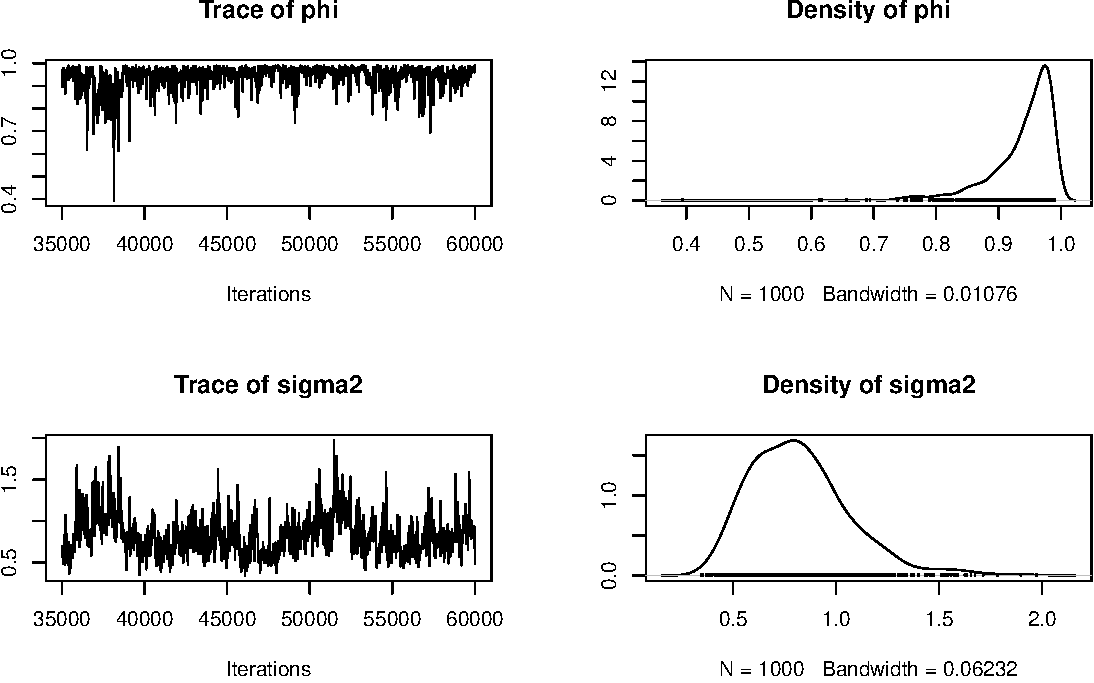
\includegraphics{Lec20_files/figure-beamer/unnamed-chunk-9-1.pdf}

\end{frame}

\begin{frame}{Predictions \& Residuals}

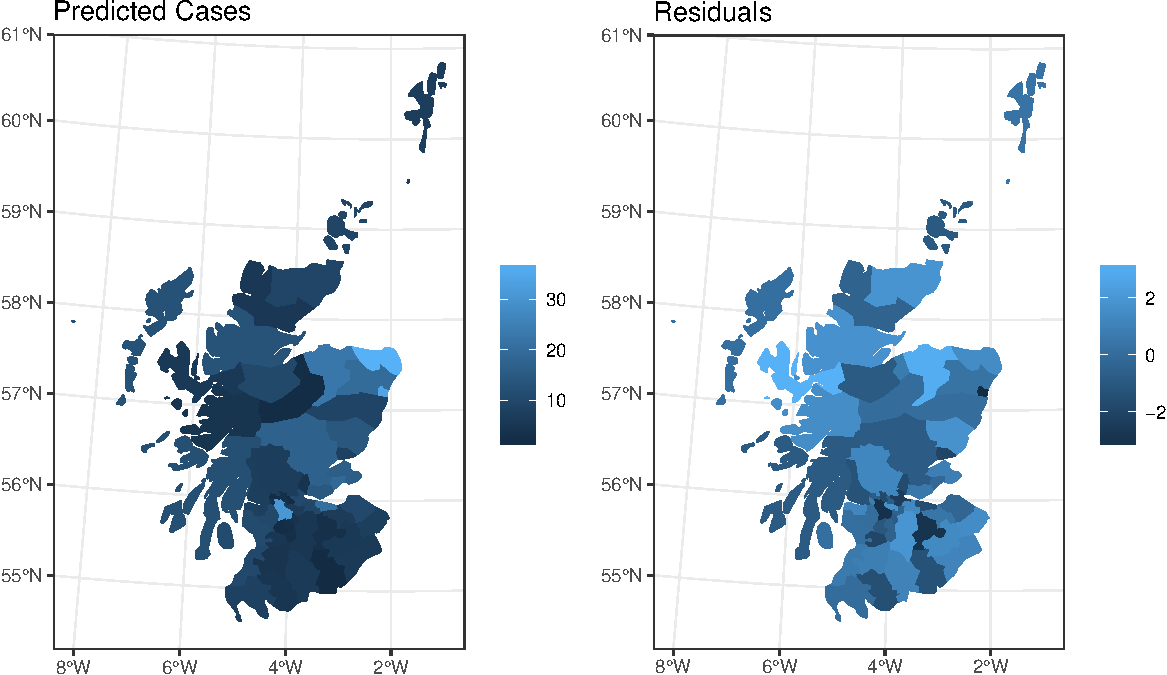
\includegraphics{Lec20_files/figure-beamer/unnamed-chunk-10-1.pdf}

\end{frame}

\begin{frame}[fragile,t]{Residuals + RMSE + Moran's I}

\begin{Shaded}
\begin{Highlighting}[]
\CommentTok{#RMSE}
\NormalTok{lip_cancer_pred}\OperatorTok{$}\NormalTok{resid }\OperatorTok\StringTok{ }\NormalTok{.}\OperatorTok{^}\DecValTok{2} \OperatorTok\StringTok{ }\KeywordTok{mean}\NormalTok{() }\OperatorTok\StringTok{ }\KeywordTok{sqrt}\NormalTok{()}
\NormalTok{## [1] 1.498675}


\CommentTok{#Moran's I}
\KeywordTok{morans_I}\NormalTok{(}\DataTypeTok{y =}\NormalTok{ lip_cancer_pred}\OperatorTok{$}\NormalTok{resid, }\DataTypeTok{w =} \KeywordTok{diag}\NormalTok{(}\KeywordTok{rowSums}\NormalTok{(W)) }\OperatorTok\StringTok{ }\NormalTok{W)}
\NormalTok{## [1] 0.05661104}

\NormalTok{ape}\OperatorTok{::}\KeywordTok{Moran.I}\NormalTok{(lip_cancer_pred}\OperatorTok{$}\NormalTok{resid, }
             \DataTypeTok{weight =} \KeywordTok{diag}\NormalTok{(}\KeywordTok{rowSums}\NormalTok{(W)) }\OperatorTok\StringTok{ }\NormalTok{W) }\OperatorTok\StringTok{ }\KeywordTok{str}\NormalTok{()}
\NormalTok{## List of 4}
\NormalTok{##  $ observed: num 0.0642}
\NormalTok{##  $ expected: num -0.0182}
\NormalTok{##  $ sd      : num 0.0803}
\NormalTok{##  $ p.value : num 0.305}
\end{Highlighting}
\end{Shaded}

\end{frame}

\section{Point Referenced Data}\label{point-referenced-data}

\begin{frame}{Example - PM2.5 from CSN}

The Chemical Speciation Network are a series of air quality monitors run
by EPA (221 locations in 2007). We'll look at a subset of the data from
Nov 11th, 2007 (n=191) for just PM2.5.

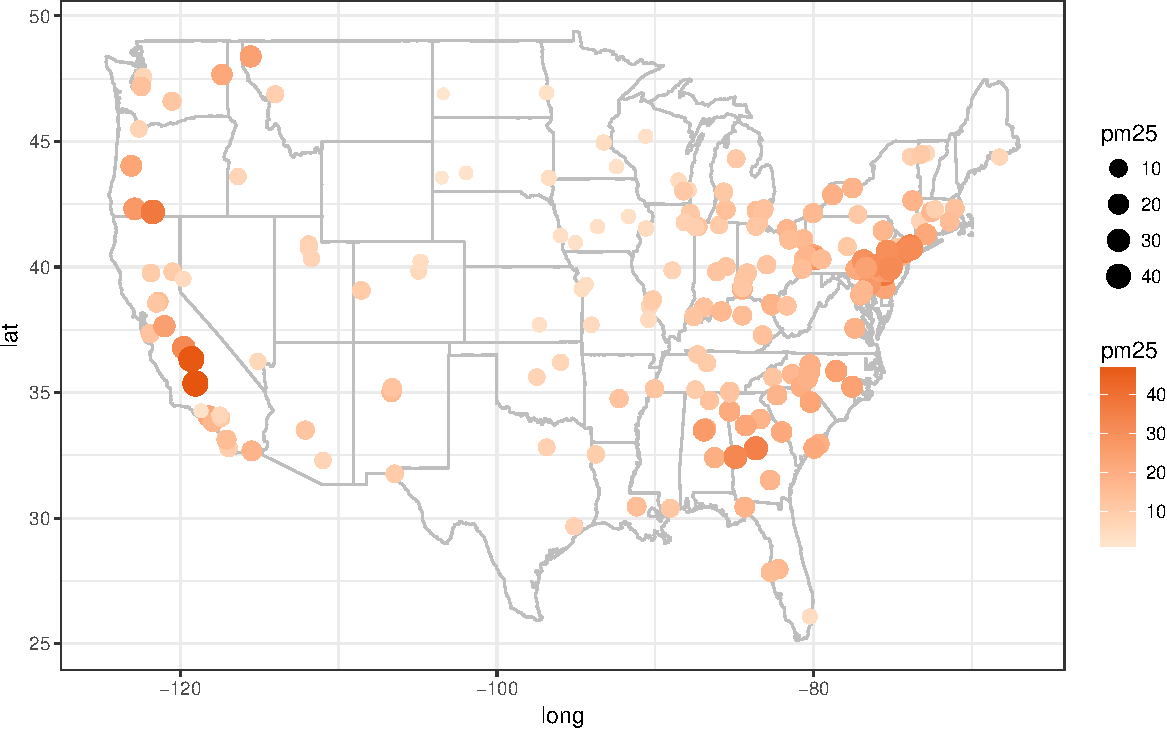
\includegraphics{Lec20_files/figure-beamer/unnamed-chunk-12-1.pdf}

\end{frame}

\begin{frame}[fragile]{}

\begin{Shaded}
\begin{Highlighting}[]
\NormalTok{csn}
\NormalTok{## # A tibble: 191 × 5}
\NormalTok{##        site  longitude latitude       date     pm25}
\NormalTok{##       <int>      <dbl>    <dbl>     <dttm>    <dbl>}
\NormalTok{## 1  10730023  -86.81500 33.55306 2007-11-14 19.43555}
\NormalTok{## 2  10732003  -86.92417 33.49972 2007-11-14 26.40000}
\NormalTok{## 3  10890014  -86.58637 34.68767 2007-11-14 13.40000}
\NormalTok{## 4  11011002  -86.25637 32.40712 2007-11-14 19.70000}
\NormalTok{## 5  11130001  -84.99917 32.47639 2007-11-14 22.60000}
\NormalTok{## 6  40139997 -112.09577 33.50383 2007-11-14 12.30000}
\NormalTok{## 7  40191028 -110.98230 32.29515 2007-11-14  7.20000}
\NormalTok{## 8  51190007  -92.28130 34.75619 2007-11-14 12.70000}
\NormalTok{## 9  60070002 -121.84222 39.75750 2007-11-14 10.00000}
\NormalTok{## 10 60190008 -119.77222 36.78139 2007-11-14 32.26205}
\NormalTok{## # ... with 181 more rows}
\end{Highlighting}
\end{Shaded}

\end{frame}

\begin{frame}{Aside - Splines}

\begin{center}
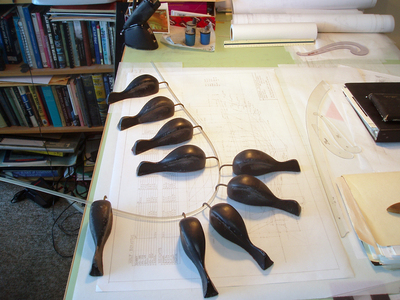
\includegraphics[width=0.49\textwidth]{figs/spline1.png}
$~$
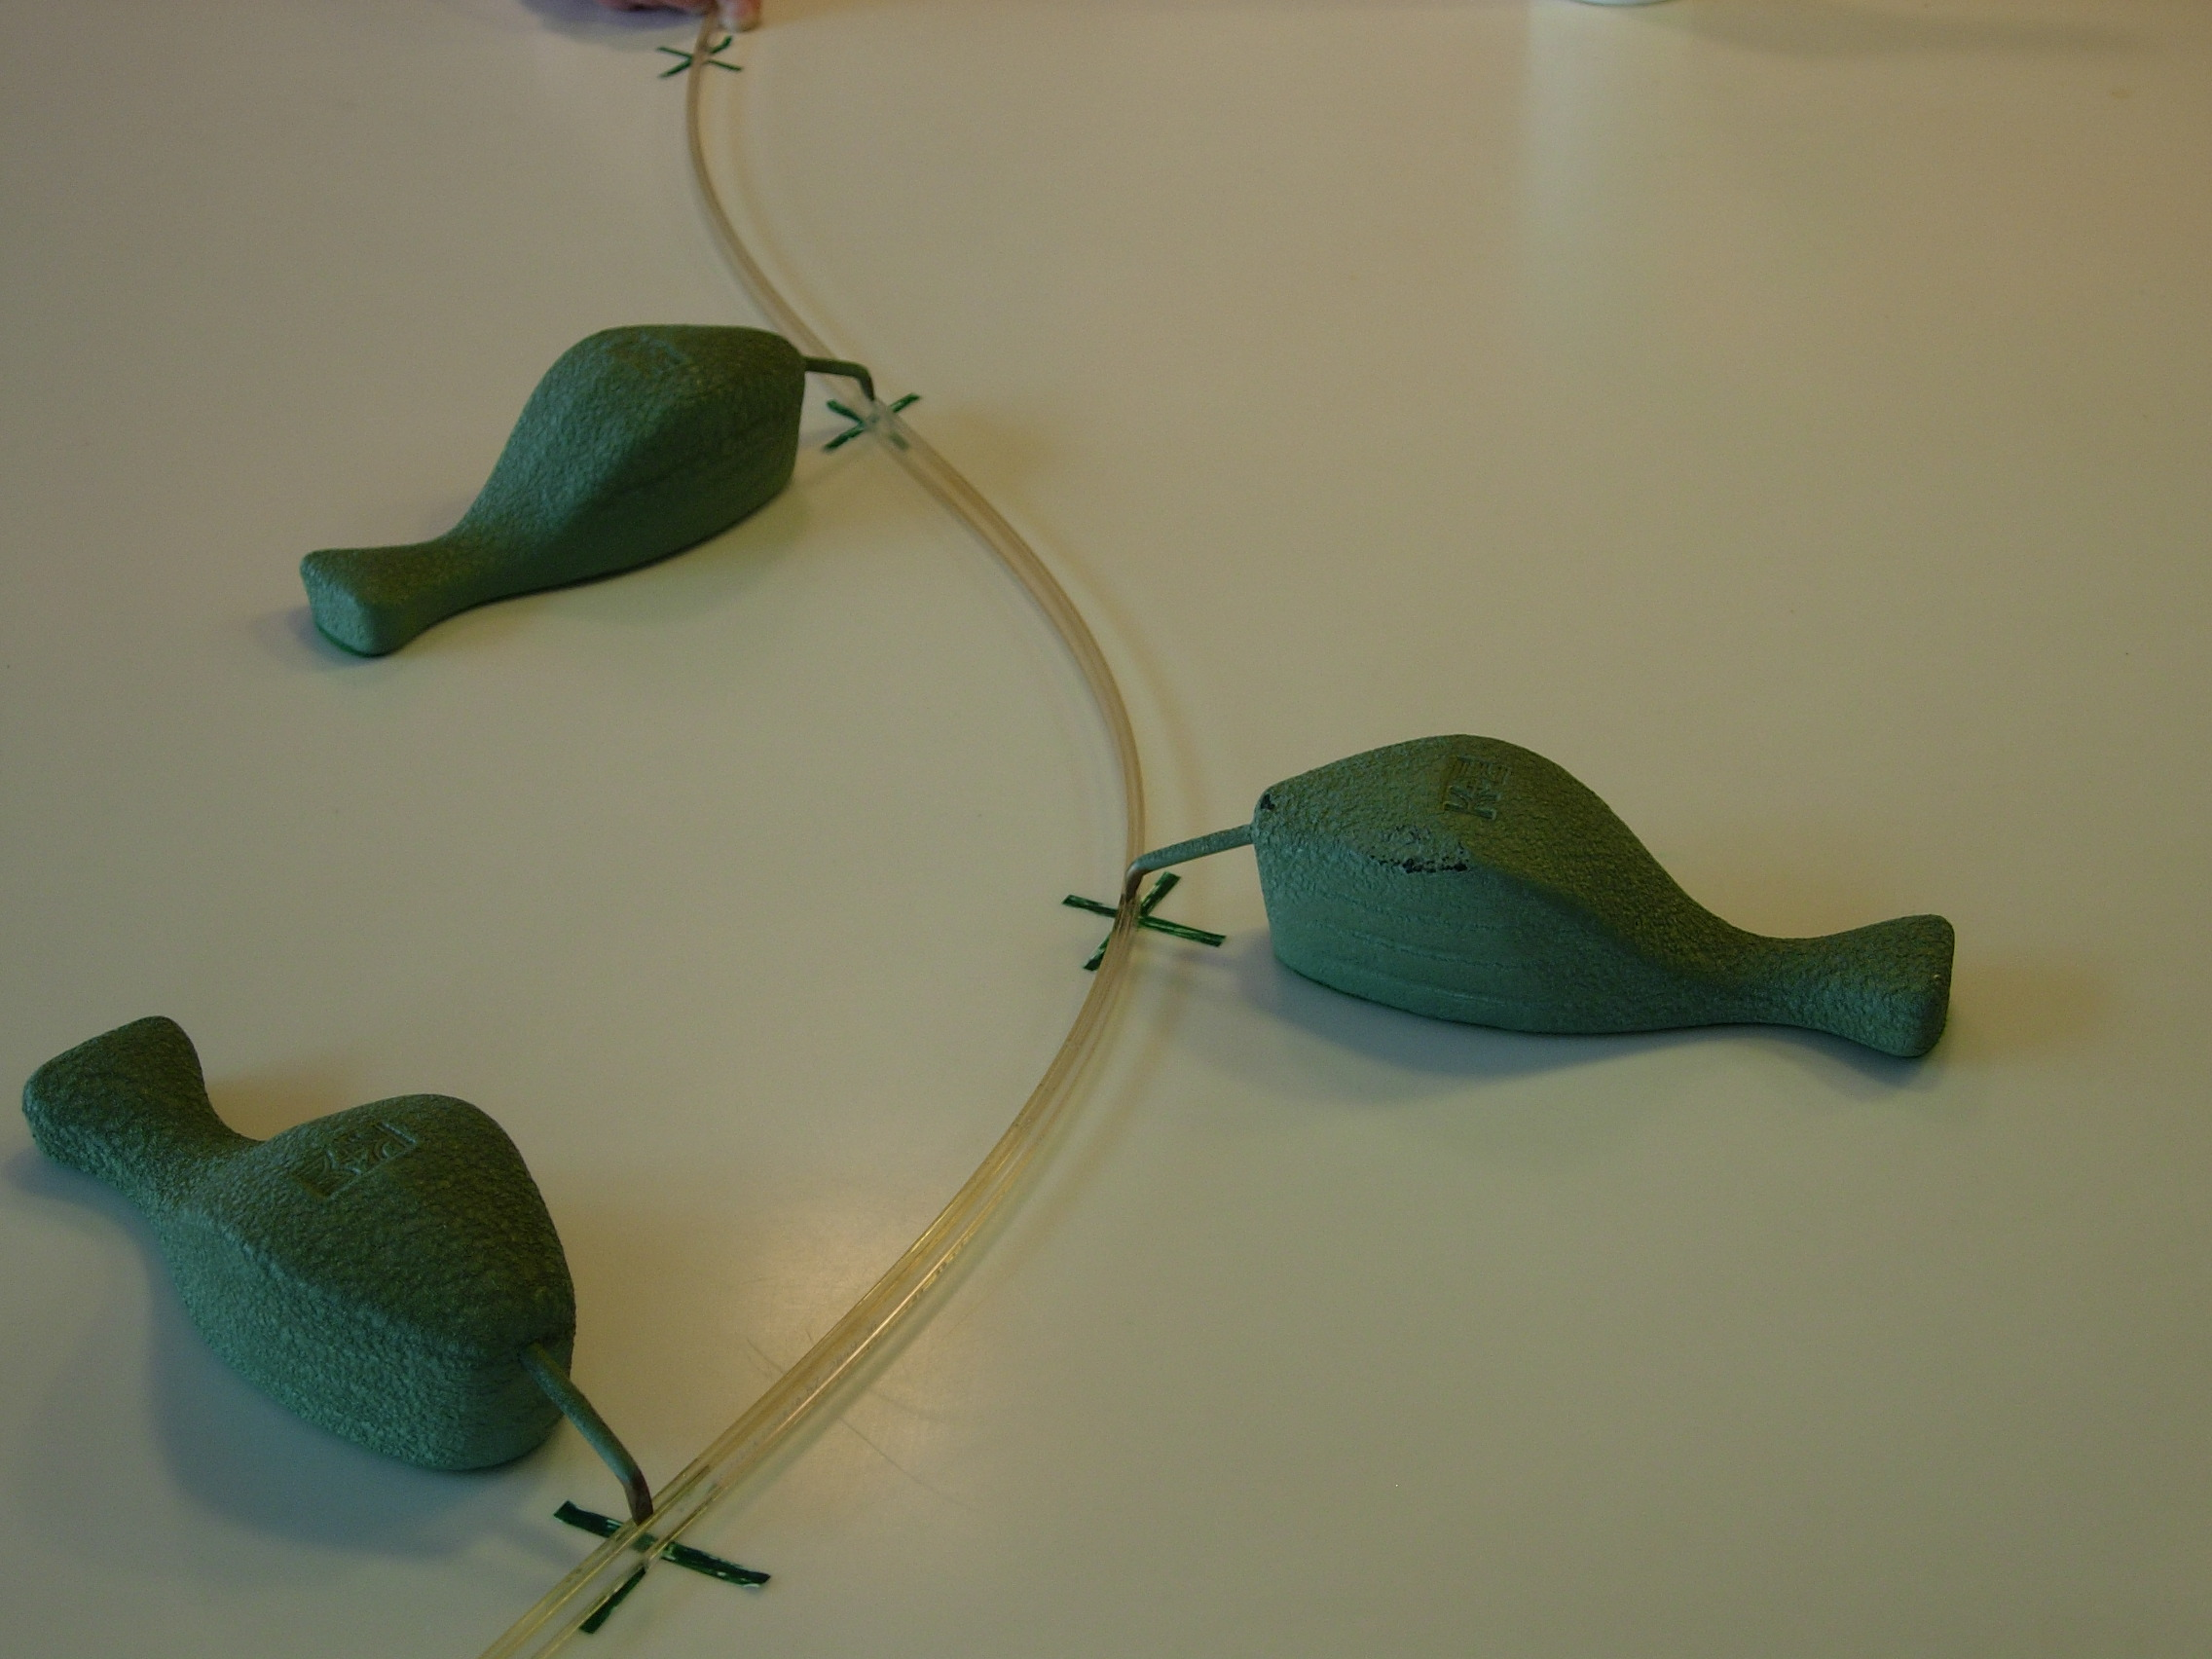
\includegraphics[width=0.49\textwidth]{figs/spline2.png}
\end{center}

\end{frame}

\begin{frame}[t]{Splines in 1d - Smoothing Splines}

These are a mathematical analogue to the drafting splines represented
using a penalized regression model.

\pause

We want to find a function \(f(x)\) that best fits our observed data
\(\bm{y} = y_1, \ldots, y_n\) while being as \emph{smooth} as possible.

\[ \underset{f(x)}{\arg\min} ~ \sum_{i=1}^n\left(y_i - f(x_i)\right)^2 + \lambda \int f''(x)^2 ~ dx \]

Interestingly, this minimization problem has an exact solution which is
given by a mixture of weighted natural cubic splines (cubic splines that
are linear in the tails) with knots at the observed data locations
(\(x\)s).

\end{frame}

\begin{frame}{Splines in 2d - Thin Plate Splines}

Now imagine we have observed data of the form \((x_i, y_i, z_i)\) where
we wish to predict \(z_i\) given \(x_i\) and \(y_i\) for all \(i\). We
can naturally extend the smoothing spline model in two dimensions,

\[ \underset{f(x,y)}{\arg\min} ~~ \sum_{i=1}^n (z_i-f(x_i,y_i))^2 + \lambda \int \int \left(\frac{\partial^2 f}{\partial x^2} + 2 \frac{\partial^2 f}{\partial x \, \partial y} + \frac{\partial^2 f}{\partial y^2} \right) dx\, dy\]

The solution to this equation has a natural representation using a
weighted sum of \emph{radial basis functions} with knots at the observed
data locations

\[ f(x,y) = \sum_{i=1}^n w_i ~ d(x_i,y_i)^2 \log d(x_i,y_i).  \]

\end{frame}

\begin{frame}[fragile,t]{Fitting a TPS}

\scriptoutput

\begin{Shaded}
\begin{Highlighting}[]
\KeywordTok{library}\NormalTok{(fields)}
\NormalTok{coords =}\StringTok{ }\KeywordTok{select}\NormalTok{(csn, longitude, latitude) }\OperatorTok\StringTok{ }\KeywordTok{as.matrix}\NormalTok{()}
\NormalTok{tps =}\StringTok{ }\KeywordTok{Tps}\NormalTok{(}\DataTypeTok{x =}\NormalTok{ coords, }\DataTypeTok{Y=}\NormalTok{csn}\OperatorTok{$}\NormalTok{pm25)}

\NormalTok{pm25_pred =}\StringTok{ }\NormalTok{r}
\NormalTok{pm25_pred[cells] =}\StringTok{ }\KeywordTok{predict}\NormalTok{(tps, pred_coords)}

\KeywordTok{plot}\NormalTok{(pm25_pred)}
\KeywordTok{points}\NormalTok{(coords, }\DataTypeTok{pch=}\DecValTok{16}\NormalTok{, }\DataTypeTok{cex=}\FloatTok{0.5}\NormalTok{)}
\end{Highlighting}
\end{Shaded}

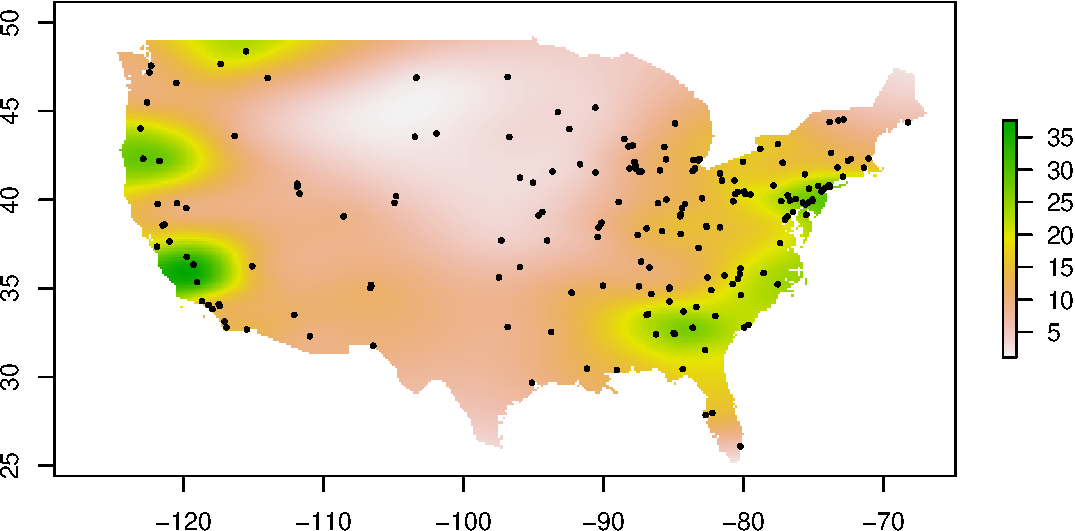
\includegraphics{Lec20_files/figure-beamer/unnamed-chunk-15-1.pdf}

\end{frame}

\section{Gaussin Process Models /
Kriging}\label{gaussin-process-models-kriging}

\begin{frame}[fragile]{Variogram}

\scriptoutput

\begin{Shaded}
\begin{Highlighting}[]
\KeywordTok{library}\NormalTok{(geoR)}
\NormalTok{coords =}\StringTok{ }\NormalTok{csn }\OperatorTok\StringTok{ }\KeywordTok{select}\NormalTok{(latitude, longitude) }\OperatorTok\StringTok{ }\KeywordTok{as.matrix}\NormalTok{()}
\NormalTok{d =}\StringTok{ }\KeywordTok{dist}\NormalTok{(coords) }\OperatorTok\StringTok{ }\KeywordTok{as.matrix}\NormalTok{()}

\KeywordTok{variog}\NormalTok{(}\DataTypeTok{coords =}\NormalTok{ coords, }\DataTypeTok{data =}\NormalTok{ csn}\OperatorTok{$}\NormalTok{pm25, }\DataTypeTok{messages =} \OtherTok{FALSE}\NormalTok{, }
       \DataTypeTok{uvec =} \KeywordTok{seq}\NormalTok{(}\DecValTok{0}\NormalTok{, }\KeywordTok{max}\NormalTok{(d)}\OperatorTok{/}\DecValTok{2}\NormalTok{, }\DataTypeTok{length.out=}\DecValTok{50}\NormalTok{)) }\OperatorTok\StringTok{ }\KeywordTok{plot}\NormalTok{()}
\end{Highlighting}
\end{Shaded}

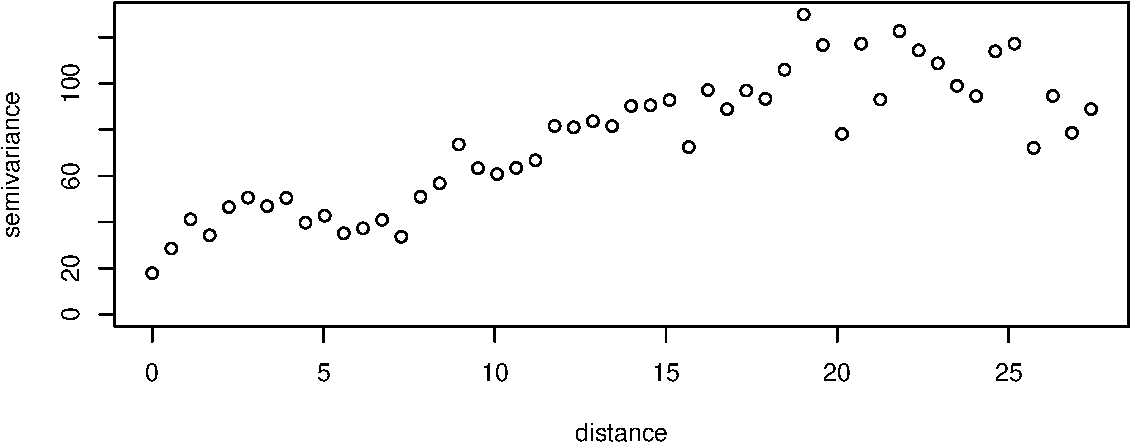
\includegraphics{Lec20_files/figure-beamer/unnamed-chunk-16-1.pdf}

\end{frame}

\begin{frame}[fragile]{}

\begin{Shaded}
\begin{Highlighting}[]
\KeywordTok{variog}\NormalTok{(}\DataTypeTok{coords =}\NormalTok{ coords, }\DataTypeTok{data =}\NormalTok{ csn}\OperatorTok{$}\NormalTok{pm25, }\DataTypeTok{messages =} \OtherTok{FALSE}\NormalTok{,}
       \DataTypeTok{uvec =} \KeywordTok{seq}\NormalTok{(}\DecValTok{0}\NormalTok{, }\KeywordTok{max}\NormalTok{(d)}\OperatorTok{/}\DecValTok{4}\NormalTok{, }\DataTypeTok{length.out=}\DecValTok{50}\NormalTok{)) }\OperatorTok\StringTok{ }\KeywordTok{plot}\NormalTok{()}
\end{Highlighting}
\end{Shaded}

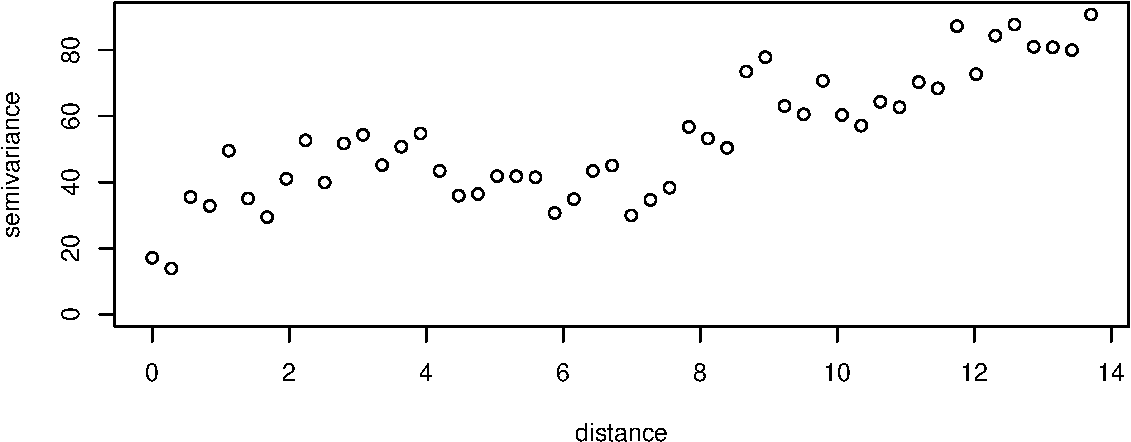
\includegraphics{Lec20_files/figure-beamer/unnamed-chunk-17-1.pdf}

\end{frame}

\begin{frame}[fragile]{Isotropy / Anisotropy}

\scriptoutput

\begin{Shaded}
\begin{Highlighting}[]
\NormalTok{v4 =}\StringTok{ }\KeywordTok{variog4}\NormalTok{(}\DataTypeTok{coords =}\NormalTok{ coords, }\DataTypeTok{data =}\NormalTok{ csn}\OperatorTok{$}\NormalTok{pm25, }\DataTypeTok{messages =} \OtherTok{FALSE}\NormalTok{,}
             \DataTypeTok{uvec =} \KeywordTok{seq}\NormalTok{(}\DecValTok{0}\NormalTok{, }\KeywordTok{max}\NormalTok{(d)}\OperatorTok{/}\DecValTok{4}\NormalTok{, }\DataTypeTok{length.out =} \DecValTok{50}\NormalTok{))}
\KeywordTok{plot}\NormalTok{(v4)}
\end{Highlighting}
\end{Shaded}

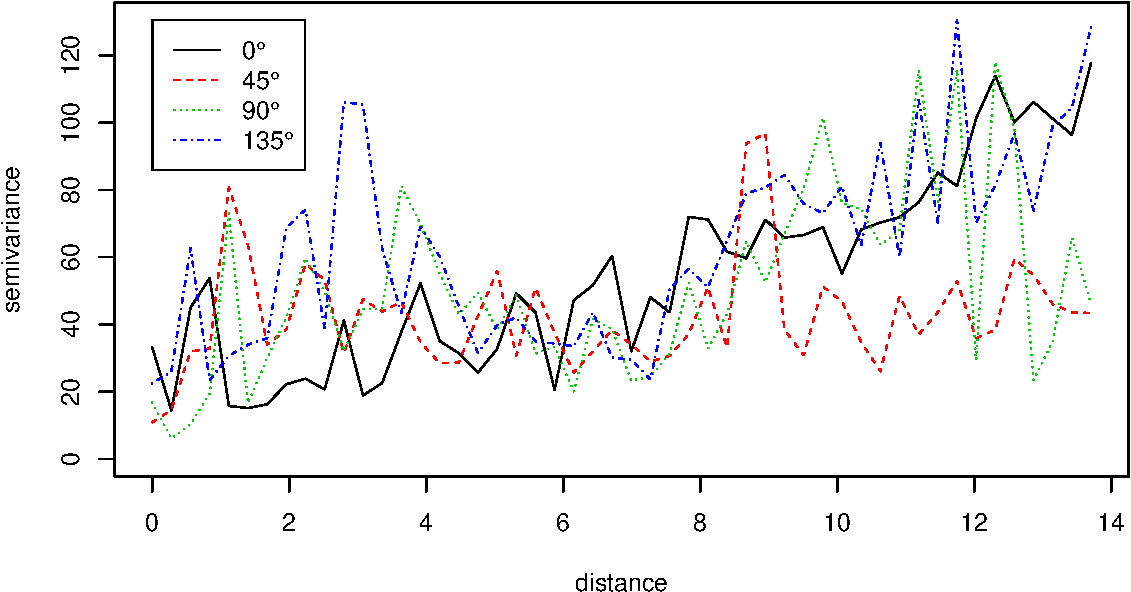
\includegraphics{Lec20_files/figure-beamer/unnamed-chunk-18-1.pdf}

\end{frame}

\begin{frame}{GP Spatial Model}

\small

If we assume that our data is \emph{stationary} and \emph{isotropic}
then we can use a Gaussian Process model to fit the data. We will assume
an exponential covariance structure.

\[ \bm{y} \sim \mathcal{N}(\mu\bm{1},~\Sigma) \]
\[ \{\Sigma\}_{ij} = \sigma^2 \exp(- r \, \lVert s_i - s_j\lVert) + \sigma^2_n \, 1_{i=j} \]

\pause

we can also view this as a spatial random effects model where

\[ y(\bm{s}) = \mu(\bm{s}) + w(\bm{s}) + \epsilon(\bm{s}) \]
\[ w(\bm{s}) \sim \mathcal{N}(0,\Sigma') \]
\[ \epsilon(s_i) \sim \mathcal{N}(0,\sigma^2_n) \]
\[ \{\Sigma'\}_{ij} = \sigma^2 \exp(- r \, \lVert s_i - s_j\lVert) \]

\end{frame}

\begin{frame}[fragile]{Fitting with \texttt{spBayes}}

\begin{Shaded}
\begin{Highlighting}[]
\KeywordTok{library}\NormalTok{(spBayes)}

\NormalTok{n =}\StringTok{ }\KeywordTok{nrow}\NormalTok{(csn)}
\NormalTok{n_samp =}\StringTok{ }\DecValTok{20000}
\NormalTok{coords =}\StringTok{ }\KeywordTok{select}\NormalTok{(csn, longitude, latitude) }\OperatorTok\StringTok{ }\KeywordTok{as.matrix}\NormalTok{()}
\NormalTok{max_range =}\StringTok{ }\KeywordTok{max}\NormalTok{(}\KeywordTok{dist}\NormalTok{(coords)) }\OperatorTok{/}\StringTok{ }\DecValTok{4}


\NormalTok{starting =}\StringTok{ }\KeywordTok{list}\NormalTok{(}\DataTypeTok{phi =} \DecValTok{3}\OperatorTok{/}\DecValTok{3}\NormalTok{, }\DataTypeTok{sigma.sq =} \DecValTok{33}\NormalTok{, }\DataTypeTok{tau.sq =} \DecValTok{17}\NormalTok{)}
\NormalTok{tuning =}\StringTok{ }\KeywordTok{list}\NormalTok{(}\StringTok{"phi"}\NormalTok{=}\FloatTok{0.1}\NormalTok{, }\StringTok{"sigma.sq"}\NormalTok{=}\FloatTok{0.1}\NormalTok{, }\StringTok{"tau.sq"}\NormalTok{=}\FloatTok{0.1}\NormalTok{)}
\NormalTok{priors =}\StringTok{ }\KeywordTok{list}\NormalTok{(}
  \DataTypeTok{beta.Norm =} \KeywordTok{list}\NormalTok{(}\DecValTok{0}\NormalTok{, }\DecValTok{1000}\NormalTok{), }
  \DataTypeTok{phi.Unif =} \KeywordTok{c}\NormalTok{(}\DecValTok{3}\OperatorTok{/}\NormalTok{max_range, }\DecValTok{6}\NormalTok{), }
  \DataTypeTok{sigma.sq.IG =} \KeywordTok{c}\NormalTok{(}\DecValTok{2}\NormalTok{, }\DecValTok{2}\NormalTok{), }
  \DataTypeTok{tau.sq.IG =} \KeywordTok{c}\NormalTok{(}\DecValTok{2}\NormalTok{, }\DecValTok{2}\NormalTok{)}
\NormalTok{)}
\end{Highlighting}
\end{Shaded}

\end{frame}

\begin{frame}[fragile]{}

\scriptoutput

\begin{Shaded}
\begin{Highlighting}[]
\NormalTok{m =}\StringTok{ }\KeywordTok{spLM}\NormalTok{(pm25 }\OperatorTok{~}\StringTok{ }\DecValTok{1}\NormalTok{, }\DataTypeTok{data =}\NormalTok{ csn, }\DataTypeTok{coords =}\NormalTok{ coords, }\DataTypeTok{starting =}\NormalTok{ starting, }\DataTypeTok{priors =}\NormalTok{ priors, }
         \DataTypeTok{cov.model =} \StringTok{"exponential"}\NormalTok{, }\DataTypeTok{n.samples =}\NormalTok{ n_samp, }\DataTypeTok{tuning =}\NormalTok{ tuning,}
         \DataTypeTok{n.report =}\NormalTok{ n_samp}\OperatorTok{/}\DecValTok{2}\NormalTok{)}
\NormalTok{## ----------------------------------------}
\NormalTok{##  General model description}
\NormalTok{## ----------------------------------------}
\NormalTok{## Model fit with 191 observations.}
\NormalTok{## }
\NormalTok{## Number of covariates 1 (including intercept if specified).}
\NormalTok{## }
\NormalTok{## Using the exponential spatial correlation model.}
\NormalTok{## }
\NormalTok{## Number of MCMC samples 20000.}
\NormalTok{## }
\NormalTok{## Priors and hyperpriors:}
\NormalTok{##  beta normal:}
\NormalTok{##  mu: 0.000   }
\NormalTok{##  cov:}
\NormalTok{##  1000.000    }
\NormalTok{## }
\NormalTok{##  sigma.sq IG hyperpriors shape=2.00000 and scale=2.00000}
\NormalTok{##  tau.sq IG hyperpriors shape=2.00000 and scale=2.00000}
\NormalTok{##  phi Unif hyperpriors a=0.21888 and b=6.00000}
\NormalTok{## -------------------------------------------------}
\NormalTok{##      Sampling}
\NormalTok{## -------------------------------------------------}
\NormalTok{## Sampled: 10000 of 20000, 50.00%}
\NormalTok{## Report interval Metrop. Acceptance rate: 33.25%}
\NormalTok{## Overall Metrop. Acceptance rate: 33.25%}
\NormalTok{## -------------------------------------------------}
\NormalTok{## Sampled: 20000 of 20000, 100.00%}
\NormalTok{## Report interval Metrop. Acceptance rate: 33.53%}
\NormalTok{## Overall Metrop. Acceptance rate: 33.39%}
\NormalTok{## -------------------------------------------------}
\end{Highlighting}
\end{Shaded}

\end{frame}

\begin{frame}[fragile]{}

\scriptoutput

\begin{Shaded}
\begin{Highlighting}[]
\NormalTok{m =}\StringTok{ }\KeywordTok{spRecover}\NormalTok{(m, }\DataTypeTok{start=}\NormalTok{n_samp}\OperatorTok{/}\DecValTok{2}\OperatorTok{+}\DecValTok{1}\NormalTok{, }\DataTypeTok{thin =}\NormalTok{ (n_samp}\OperatorTok{/}\DecValTok{2}\NormalTok{)}\OperatorTok{/}\DecValTok{1000}\NormalTok{)}
\NormalTok{## -------------------------------------------------}
\NormalTok{##      Recovering beta and w}
\NormalTok{## -------------------------------------------------}
\NormalTok{## Sampled: 99 of 1000, 9.90%}
\NormalTok{## Sampled: 199 of 1000, 19.90%}
\NormalTok{## Sampled: 299 of 1000, 29.90%}
\NormalTok{## Sampled: 399 of 1000, 39.90%}
\NormalTok{## Sampled: 499 of 1000, 49.90%}
\NormalTok{## Sampled: 599 of 1000, 59.90%}
\NormalTok{## Sampled: 699 of 1000, 69.90%}
\NormalTok{## Sampled: 799 of 1000, 79.90%}
\NormalTok{## Sampled: 899 of 1000, 89.90%}
\NormalTok{## Sampled: 999 of 1000, 99.90%}
\end{Highlighting}
\end{Shaded}

\end{frame}

\begin{frame}[fragile]{Parameter values}

\begin{Shaded}
\begin{Highlighting}[]
\NormalTok{m}\OperatorTok{$}\NormalTok{p.theta.recover.samples }\OperatorTok\StringTok{ }\KeywordTok{mcmc}\NormalTok{() }\OperatorTok\StringTok{ }\KeywordTok{plot}\NormalTok{()}
\end{Highlighting}
\end{Shaded}

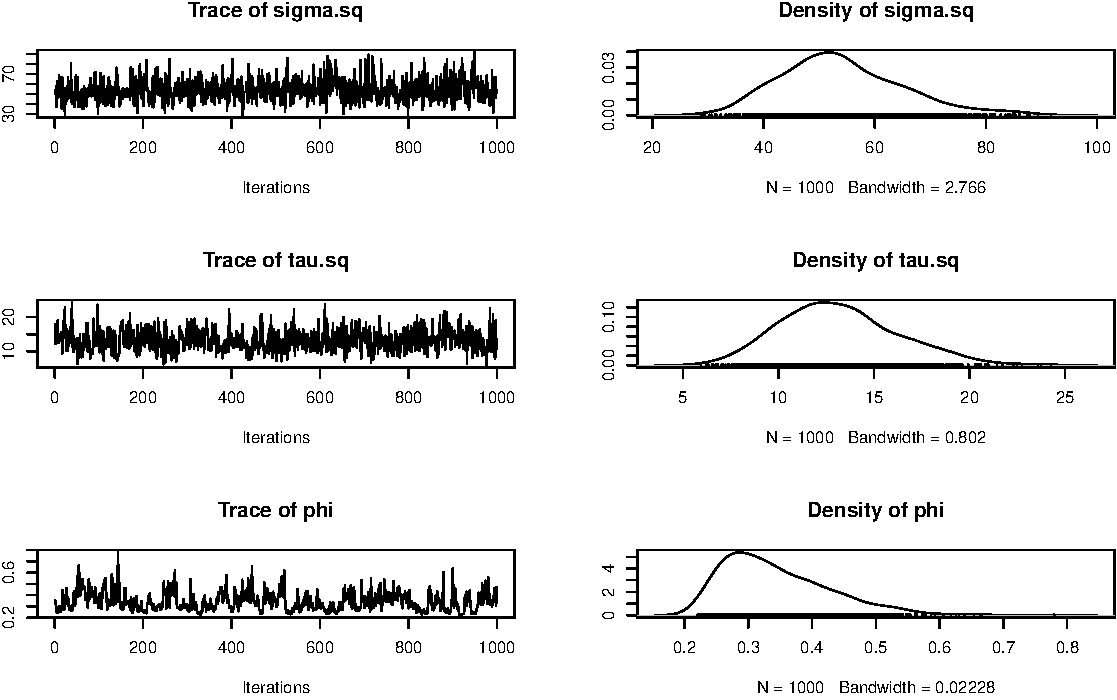
\includegraphics{Lec20_files/figure-beamer/unnamed-chunk-22-1.pdf}

\end{frame}

\begin{frame}[fragile]{}

\begin{Shaded}
\begin{Highlighting}[]
\NormalTok{m}\OperatorTok{$}\NormalTok{p.beta.recover.samples }\OperatorTok\StringTok{ }\KeywordTok{mcmc}\NormalTok{() }\OperatorTok\StringTok{ }\KeywordTok{plot}\NormalTok{()}
\end{Highlighting}
\end{Shaded}

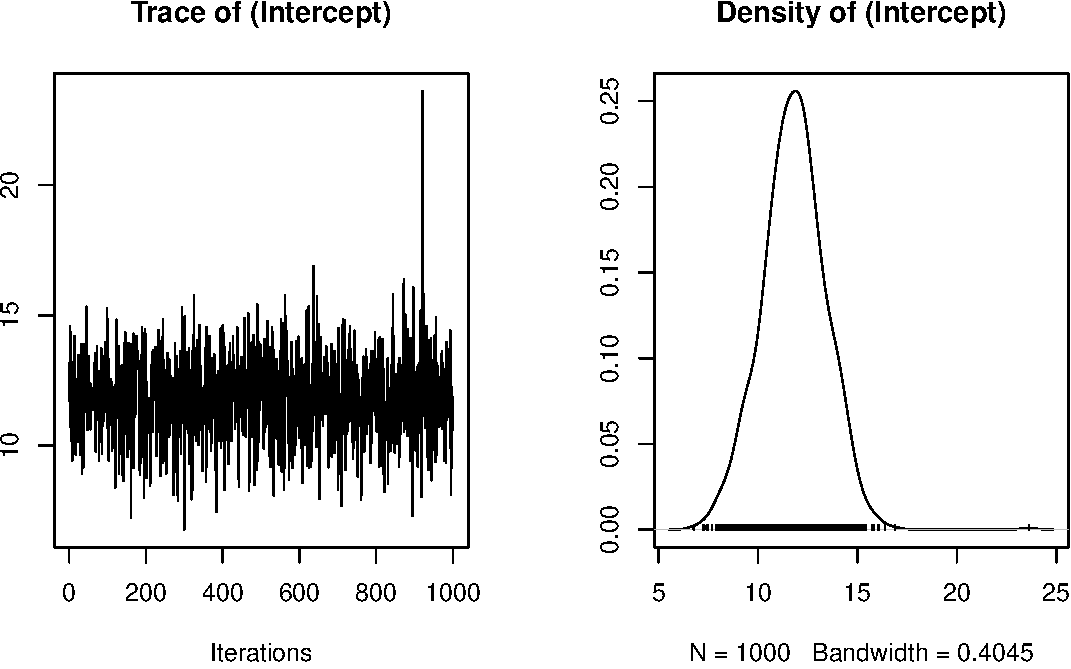
\includegraphics{Lec20_files/figure-beamer/unnamed-chunk-23-1.pdf}

\end{frame}

\begin{frame}[fragile]{Predictions}

\begin{Shaded}
\begin{Highlighting}[]
\NormalTok{m_pred =}\StringTok{ }\KeywordTok{spPredict}\NormalTok{(m, pred_coords, }\DataTypeTok{pred.covars =} \KeywordTok{matrix}\NormalTok{(}\DecValTok{1}\NormalTok{, }\DataTypeTok{nrow=}\KeywordTok{nrow}\NormalTok{(pred_coords)), }
                   \DataTypeTok{start=}\NormalTok{n_samp}\OperatorTok{/}\DecValTok{2}\OperatorTok{+}\DecValTok{1}\NormalTok{, }\DataTypeTok{thin=}\NormalTok{(n_samp}\OperatorTok{/}\DecValTok{2}\NormalTok{)}\OperatorTok{/}\DecValTok{1000}\NormalTok{)}
\NormalTok{## ----------------------------------------}
\NormalTok{##  General model description}
\NormalTok{## ----------------------------------------}
\NormalTok{## Model fit with 191 observations.}
\NormalTok{## }
\NormalTok{## Prediction at 900 locations.}
\NormalTok{## }
\NormalTok{## Number of covariates 1 (including intercept if specified).}
\NormalTok{## }
\NormalTok{## Using the exponential spatial correlation model.}
\NormalTok{## }
\NormalTok{## -------------------------------------------------}
\NormalTok{##      Sampling}
\NormalTok{## -------------------------------------------------}
\NormalTok{## Sampled: 100 of 1000, 9.90%}
\NormalTok{## Sampled: 200 of 1000, 19.90%}
\NormalTok{## Sampled: 300 of 1000, 29.90%}
\NormalTok{## Sampled: 400 of 1000, 39.90%}
\NormalTok{## Sampled: 500 of 1000, 49.90%}
\NormalTok{## Sampled: 600 of 1000, 59.90%}
\NormalTok{## Sampled: 700 of 1000, 69.90%}
\NormalTok{## Sampled: 800 of 1000, 79.90%}
\NormalTok{## Sampled: 900 of 1000, 89.90%}
\NormalTok{## Sampled: 1000 of 1000, 99.90%}
\NormalTok{m_pred_summary =}\StringTok{ }\KeywordTok{post_summary}\NormalTok{(}\KeywordTok{t}\NormalTok{(m_pred}\OperatorTok{$}\NormalTok{p.y.predictive.samples))}
\end{Highlighting}
\end{Shaded}

\end{frame}

\begin{frame}[fragile]{}

\begin{Shaded}
\begin{Highlighting}[]
\NormalTok{splm_pm25_pred =}\StringTok{ }\NormalTok{r}
\NormalTok{splm_pm25_pred[cells] =}\StringTok{ }\NormalTok{m_pred_summary}\OperatorTok{$}\NormalTok{post_mean}

\KeywordTok{plot}\NormalTok{(splm_pm25_pred)}
\KeywordTok{points}\NormalTok{(coords, }\DataTypeTok{pch=}\DecValTok{16}\NormalTok{, }\DataTypeTok{cex=}\FloatTok{0.5}\NormalTok{)}
\end{Highlighting}
\end{Shaded}

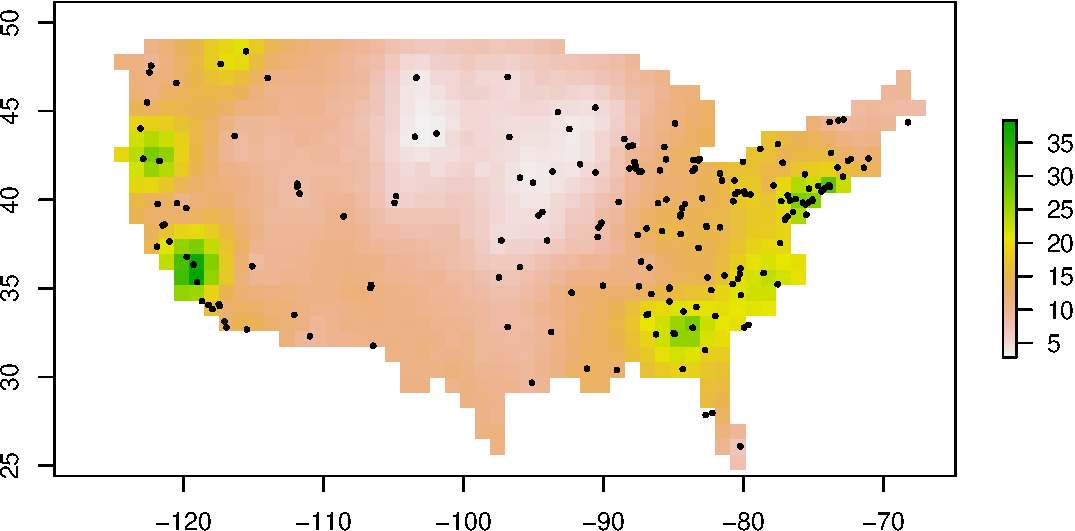
\includegraphics{Lec20_files/figure-beamer/unnamed-chunk-26-1.pdf}

\end{frame}

\begin{frame}[fragile]{JAGs Model}

\begin{verbatim}
## model{
##   for(i in 1:length(y)){
##     y[i] ~ dnorm(beta + w[i], tau)
##     mu_w[i] <- 0
##   }
##  
##   for(i in 1:length(y)){
##     for(j in 1:length(y)){
##       Sigma_w[i,j] <- sigma2_w * exp(-phi * d[i,j])
##     }
##   }
##   Sigma_w_inv <- inverse(Sigma_w)
##   w ~ dmnorm(mu_w, Sigma_w_inv)
## 
##   beta ~ dnorm(0, 1/1000)
##   sigma2_w ~ dgamma(2, 2)
##   sigma2 ~ dgamma(2, 2)
##   tau <- 1/sigma2
##   phi ~ dunif(3/14, 6)
## }
\end{verbatim}

\end{frame}

\begin{frame}{}

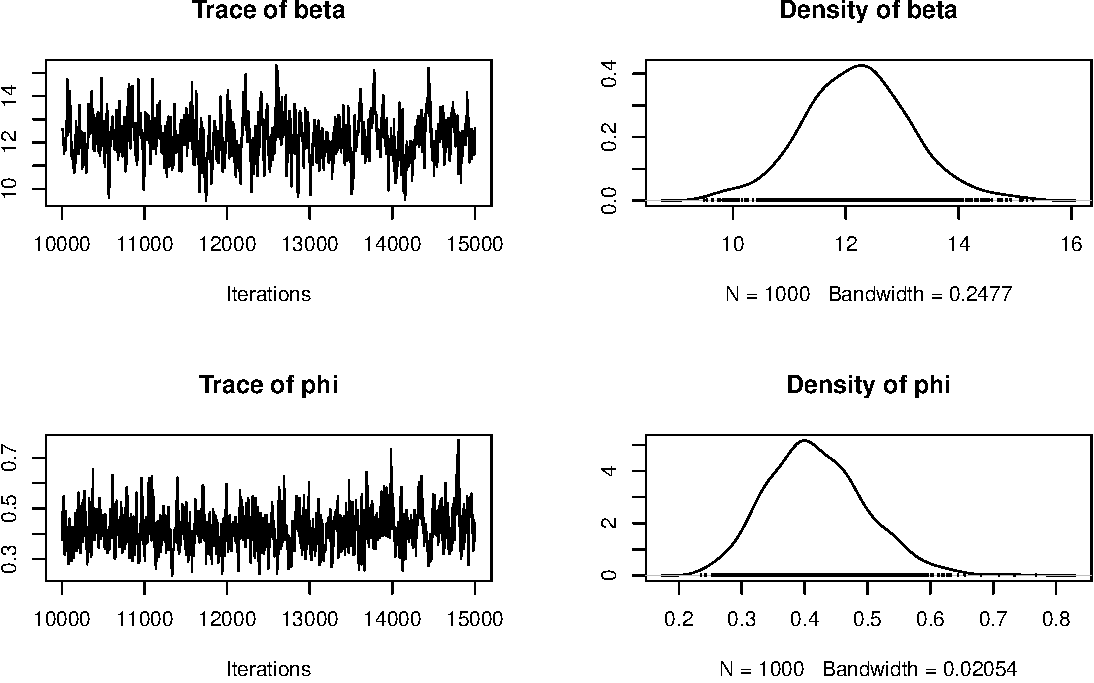
\includegraphics{Lec20_files/figure-beamer/unnamed-chunk-29-1.pdf}

\end{frame}

\begin{frame}{}

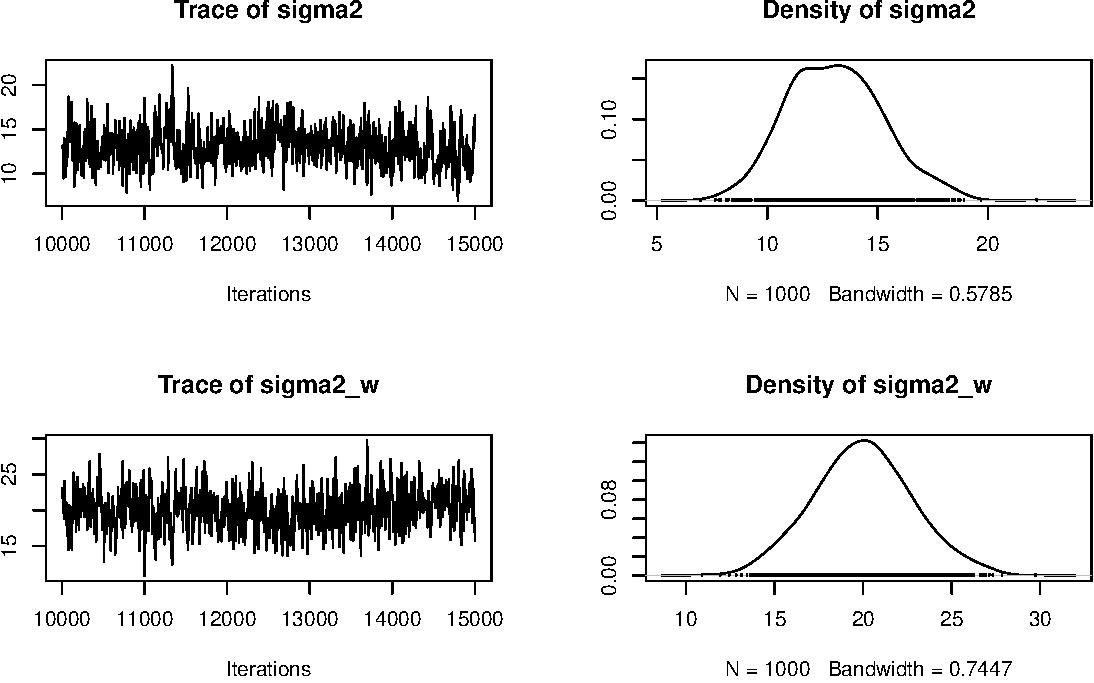
\includegraphics{Lec20_files/figure-beamer/unnamed-chunk-30-1.pdf}

\end{frame}

\end{document}
